\documentclass[a4paper,12pt,twoside]{report}
\usepackage[left=2cm,right=2cm,top=2cm,bottom=3cm]{geometry}
\usepackage[spanish]{babel}
\usepackage[utf8]{inputenc}
\usepackage{svg}
\usepackage{graphicx}


\usepackage{graphicx}
\usepackage{verbatim}
\usepackage{latexsym}
\usepackage{mathchars}
\usepackage{setspace}
\usepackage{tikz}
\usepackage{booktabs}
\usepackage{rotating}
\usepackage{tabularx}
\usepackage{lscape} 
\usepackage{tipa}
\usepackage{float}
\usepackage{url}
% \usepackage{apacite}
\usetikzlibrary{positioning}

\setlength{\parskip}{\medskipamount}  % a little space before a \par
\setlength{\parindent}{0pt}	      % don't indent first lines of paragraphs
%UHEAD.STY  If this is included after \documentstyle{report}, it adds
% an underlined heading style to the LaTeX report style.
% \pagestyle{uheadings} will put underlined headings at the top
% of each page. The right page headings are the Chapter titles and
% the left page titles are supplied by \def\lefthead{text}.

% Ted Shapin, Dec. 17, 1986

\makeatletter
\def\chapapp2{Chapter}

\def\appendix{\par
 \setcounter{chapter}{0}
 \setcounter{section}{0}
 \def\chapapp2{Appendix}
 \def\@chapapp{Appendix}
 \def\thechapter{\Alph{chapter}}}

\def\ps@uheadings{\let\@mkboth\markboth
% modifications
\def\@oddhead{\protect\underline{\protect\makebox[\textwidth][l]
		{\sl\rightmark\hfill\rm\thepage}}}
\def\@oddfoot{}
\def\@evenfoot{}
\def\@evenhead{\protect\underline{\protect\makebox[\textwidth][l]
		{\rm\thepage\hfill\sl\leftmark}}}
% end of modifications
\def\chaptermark##1{\markboth {\ifnum \c@secnumdepth >\m@ne
 \chapapp2\ \thechapter. \ \fi ##1}{}}%
\def\sectionmark##1{\markright {\ifnum \c@secnumdepth >\z@
   \thesection. \ \fi ##1}}}
\makeatother
%%From: marcel@cs.caltech.edu (Marcel van der Goot)
%%Newsgroups: comp.text.tex
%%Subject: illegal modification of boxit.sty
%%Date: 28 Feb 92 01:10:02 GMT
%%Organization: California Institute of Technology (CS dept)
%%Nntp-Posting-Host: andromeda.cs.caltech.edu
%%
%%
%%Quite some time ago I posted a file boxit.sty; maybe it made it
%%to some archives, although I don't recall submitting it. It defines
%%	\begin{boxit}
%%	...
%%	\end{boxit}
%%to draw a box around `...', where the `...' can contain other
%%environments (e.g., a verbatim environment). Unfortunately, it had
%%a problem: it did not work if you used it in paragraph mode, i.e., it
%%only worked if there was an empty line in front of \begin{boxit}.
%%Luckily, that is easily corrected.
%%
%%HOWEVER, apparently someone noticed the problem, tried to correct it,
%%and then distributed this modified version. That would be fine with me,
%%except that:
%%1. There was no note in the file about this modification, it only has my
%%   name in it.
%%2. The modification is wrong: now it only works if there is *no* empty
%%   line in front of \begin{boxit}. In my opinion this bug is worse than
%%   the original one.
%%
%%In particular, the author of this modification tried to force an empty
%%line by inserting a `\\' in the definition of \Beginboxit. If you have
%%a version of boxit.sty with a `\\', please delete it. If you have my
%%old version of boxit.sty, please also delete it. Below is an improved
%%version.
%%
%%Thanks to Joe Armstrong for drawing my attention to the bug and to the
%%illegal version.
%%
%%                                          Marcel van der Goot
%% .---------------------------------------------------------------
%% | Blauw de viooltjes,                    marcel@cs.caltech.edu
%% |    Rood zijn de rozen;
%% | Een rijm kan gezet
%% |    Met plaksel en dozen.
%% |


% boxit.sty
% version: 27 Feb 1992
%
% Defines a boxit environment, which draws lines around its contents.
% Usage:
%   \begin{boxit}
%	... (text you want to be boxed, can contain other environments)
%   \end{boxit}
%
% The width of the box is the width of the contents.
% The boxit* environment behaves the same, except that the box will be
% at least as wide as a normal paragraph.
%
% The reason for writing it this way (rather than with the \boxit#1 macro
% from the TeXbook), is that now you can box verbatim text, as in
%   \begin{boxit}
%   \begin{verbatim}
%   this better come out in boxed verbatim mode ...
%   \end{verbatim}
%   \end{boxit}
%
%						Marcel van der Goot
%						marcel@cs.caltech.edu
%

\def\Beginboxit
   {\par
    \vbox\bgroup
	   \hrule
	   \hbox\bgroup
		  \vrule \kern1.2pt %
		  \vbox\bgroup\kern1.2pt
   }

\def\Endboxit{%
			      \kern1.2pt
		       \egroup
		  \kern1.2pt\vrule
		\egroup
	   \hrule
	 \egroup
   }	

\newenvironment{boxit}{\Beginboxit}{\Endboxit}
\newenvironment{boxit*}{\Beginboxit\hbox to\hsize{}}{\Endboxit}
\pagestyle{empty}

\setlength{\parskip}{2ex plus 0.5ex minus 0.2ex}
\setlength{\parindent}{0pt}

\makeatletter  %to avoid error messages generated by "\@". Makes Latex treat "@" like a letter

\linespread{1.5}
\def\submitdate#1{\gdef\@submitdate{#1}}

\def\maketitle{
  \begin{titlepage}{
    %\linespread{1.5}
    \Large Universidad del Valle \\
    %\linebreak
    Facultad de Ingeniería
    %\linebreak
    Escuela de Ingeniería de Sistemas y Computación \\
    
    \rm
    \vskip 3in
    \Large \bf \@title \par
  }
  \vskip 0.3in
  \par
  {\Large \@author}
  \\
  \\
  {\Large 201802679}\\
  \\
  {\large mauricio.collazos@correounivalle.edu.co}
  \vskip 1in
  {\large Dirigido por}\\
  {\large Raúl Ernesto Gutierrez de Piñeres Reyes Ph.D}
  \vskip 2in
  \par
  Submitted for the approval of master degree project in
  \linebreak
  Master in Engineering with emphasis in System Engineering and Computation
  \linebreak
  \@submitdate
  \vfil
  \end{titlepage}
}

\def\titlepage{
  \newpage
  \centering
  \linespread{1}
  \normalsize
  \vbox to \vsize\bgroup\vbox to 9in\bgroup
}
\def\endtitlepage{
  \par
  \kern 0pt
  \egroup
  \vss
  \egroup
  \clearpage
}

\def\abstract{
  \begin{center}{
    \large\bf Abstract}
  \end{center}
  \small
  %\def\baselinestretch{1.5}
  \linespread{1.5}
  \normalsize
}

%\def\endabstract{
  %\par
%}

\newenvironment{acknowledgements}{
  \cleardoublepage
  \begin{center}{
    \large \bf Acknowledgements}
  \end{center}
  \small
  \linespread{1.5}
  \normalsize
}{\cleardoublepage}
\def\endacknowledgements{
  \par
}

\newenvironment{dedication}{
  \cleardoublepage
  \begin{center}{
    \large \bf Dedication}
  \end{center}
  \small
  \linespread{1.5}
  \normalsize
}{\cleardoublepage}
\def\enddedication{
  \par
}

\def\preface{
    \pagenumbering{roman}
    \pagestyle{plain}
    \doublespacing
}

\def\body{
    \clearpage
    \pagestyle{uheadings}
    \tableofcontents
    \pagestyle{plain}
    \clearpage
    \pagestyle{uheadings}
    \listoftables
    \pagestyle{plain}
    \clearpage
    \pagestyle{uheadings}
    \listoffigures
    \pagestyle{plain}
    \clearpage
    \pagestyle{uheadings}
    \pagenumbering{arabic}
    \doublespacing
}

\makeatother  %to avoid error messages generated by "\@". Makes Latex treat "@" like a letter

\newcommand{\ipc}{{\sf ipc}}

\newcommand{\Prob}{\bbbp}
\newcommand{\Real}{\bbbr}
\newcommand{\real}{\Real}
\newcommand{\Int}{\bbbz}
\newcommand{\Nat}{\bbbn}

\newcommand{\NN}{{\sf I\kern-0.14emN}}   % Natural numbers
\newcommand{\ZZ}{{\sf Z\kern-0.45emZ}}   % Integers
\newcommand{\QQQ}{{\sf C\kern-0.48emQ}}   % Rational numbers
\newcommand{\RR}{{\sf I\kern-0.14emR}}   % Real numbers
\newcommand{\KK}{{\cal K}}
\newcommand{\OO}{{\cal O}}
\newcommand{\AAA}{{\bf A}}
\newcommand{\HH}{{\bf H}}
\newcommand{\II}{{\bf I}}
\newcommand{\LL}{{\bf L}}
\newcommand{\PP}{{\bf P}}
\newcommand{\PPprime}{{\bf P'}}
\newcommand{\QQ}{{\bf Q}}
\newcommand{\UU}{{\bf U}}
\newcommand{\UUprime}{{\bf U'}}
\newcommand{\zzero}{{\bf 0}}
\newcommand{\ppi}{\mbox{\boldmath $\pi$}}
\newcommand{\aalph}{\mbox{\boldmath $\alpha$}}
\newcommand{\bb}{{\bf b}}
\newcommand{\ee}{{\bf e}}
\newcommand{\mmu}{\mbox{\boldmath $\mu$}}
\newcommand{\vv}{{\bf v}}
\newcommand{\xx}{{\bf x}}
\newcommand{\yy}{{\bf y}}
\newcommand{\zz}{{\bf z}}
\newcommand{\oomeg}{\mbox{\boldmath $\omega$}}
\newcommand{\res}{{\bf res}}
\newcommand{\cchi}{{\mbox{\raisebox{.4ex}{$\chi$}}}}
%\newcommand{\cchi}{{\cal X}}
%\newcommand{\cchi}{\mbox{\Large $\chi$}}

% Logical operators and symbols
\newcommand{\imply}{\Rightarrow}
\newcommand{\bimply}{\Leftrightarrow}
\newcommand{\union}{\cup}
\newcommand{\intersect}{\cap}
\newcommand{\boolor}{\vee}
\newcommand{\booland}{\wedge}
\newcommand{\boolimply}{\imply}
\newcommand{\boolbimply}{\bimply}
\newcommand{\boolnot}{\neg}
\newcommand{\boolsat}{\!\models}
\newcommand{\boolnsat}{\!\not\models}


\newcommand{\op}[1]{\mathrm{#1}}
% \newcommand{\s}[1]{\ensuremath{\mathcal #1}}

% Properly styled differentiation and integration operators
\newcommand{\diff}[1]{\mathrm{\frac{d}{d\mathit{#1}}}}
\newcommand{\diffII}[1]{\mathrm{\frac{d^2}{d\mathit{#1}^2}}}
\newcommand{\intg}[4]{\int_{#3}^{#4} #1 \, \mathrm{d}#2}
\newcommand{\intgd}[4]{\int\!\!\!\!\int_{#4} #1 \, \mathrm{d}#2 \, \mathrm{d}#3}

% Large () brackets on different lines of an eqnarray environment
\newcommand{\Leftbrace}[1]{\left(\raisebox{0mm}[#1][#1]{}\right.}
\newcommand{\Rightbrace}[1]{\left.\raisebox{0mm}[#1][#1]{}\right)}

% Funky symobols for footnotes
\newcommand{\symbolfootnote}{\renewcommand{\thefootnote}{\fnsymbol{footnote}}}
% now add \symbolfootnote to the beginning of the document...

\newcommand{\normallinespacing}{\renewcommand{\baselinestretch}{1.5} \normalsize}
\newcommand{\mediumlinespacing}{\renewcommand{\baselinestretch}{1.2} \normalsize}
\newcommand{\narrowlinespacing}{\renewcommand{\baselinestretch}{1.0} \normalsize}
\newcommand{\bump}{\noalign{\vspace*{\doublerulesep}}}
\newcommand{\cell}{\multicolumn{1}{}{}}
\newcommand{\spann}{\mbox{span}}
\newcommand{\diagg}{\mbox{diag}}
\newcommand{\modd}{\mbox{mod}}
\newcommand{\minn}{\mbox{min}}
\newcommand{\andd}{\mbox{and}}
\newcommand{\forr}{\mbox{for}}
\newcommand{\EE}{\mbox{E}}

\newcommand{\deff}{\stackrel{\mathrm{def}}{=}}
\newcommand{\syncc}{~\stackrel{\textstyle \rhd\kern-0.57em\lhd}{\scriptstyle L}~}

\def\coop{\mbox{\large $\rhd\!\!\!\lhd$}}
\newcommand{\sync}[1]{\raisebox{-1.0ex}{$\;\stackrel{\coop}{\scriptscriptstyle
#1}\,$}}

\newtheorem{definition}{Definition}[chapter]
\newtheorem{theorem}{Theorem}[chapter]

\newcommand{\Figref}[1]{Figure~\ref{#1}}
\newcommand{\fig}[3]{
 \begin{figure}[!ht]
 \begin{center}
 \scalebox{#3}{\includegraphics{figs/#1.ps}}
 \vspace{-0.1in}
 \caption[ ]{\label{#1} #2}
 \end{center}
 \end{figure}
}

\newcommand{\figtwo}[8]{
 \begin{figure}
 \parbox[b]{#4 \textwidth}{
 \begin{center}
 \scalebox{#3}{\includegraphics{figs/#1.ps}}
 \vspace{-0.1in}
 \caption{\label{#1}#2}
 \end{center}
 }
 \hfill
 \parbox[b]{#8 \textwidth}{
 \begin{center}
 \scalebox{#7}{\includegraphics{figs/#5.ps}}
 \vspace{-0.1in}
 \caption{\label{#5}#6}
 \end{center}
 }
 \end{figure}
}


\begin{document}

%\title{\LARGE {\bf Using hybrid techniques to improve performance on forced aligners for Spanish language}\\
% \vspace*{6mm}
%}

\title{\LARGE {\bf Anotación automática de un corpus hablado de licencia abierta y larga duración para el lenguaje español}\\
 \vspace*{6mm}
}

\author{Mauricio Collazos}
\submitdate{December 2018}

\normallinespacing
\maketitle

\preface
\addcontentsline{toc}{chapter}{Abstract}

\begin{abstract}
El reconocimiento automático del habla (Automatic Speech Recognition ASR) es una subarea de la inteligencia artificial con un amplio campo de investigación en la actualidad. Muchos avances tecnológicos han sido mostrados en la industria soportados por investigación académica enfocados en el idioma inglés, pero replicar los experimentos en otros idiomas presenta problemáticas por la falta de corpus apropiados. 

% Automatic Speech Recognition is a giant subfield of Artificial Intelligence and a broad topic for research now. Many new advances have been shown in industry supported by academic research, but replicate experiments in languages different than the English language could be a problem for the lack of proper corpora. 

El idioma español cuenta con recursos de licencia abierta hablados y anotados, pero estos recursos no son adecuados ni suficientes para replicar los resultados de investigación obtenidos para el idioma inglés. Esta tesis busca crear un corpus hablado y anotado usando recursos abiertos existentes para replicar resultados obtenidos en lenguajes extranjeros.
% The Spanish language has  speech annotated data, but its annotation is not adequate to replicate existing research with the similar results. This thesis aims to create a fine grained annotated corpora for the Spanish language to replicate existing research in foreigns languages.
% Text of the Abstract.

% Información clara y concisa de la idea del proyecto.
% • Exponga brevemente los antecedentes, el problema y la solución propuesta.
% • Exponga brevemente los resultados esperados y el impacto de ellos.
% • Lo novedoso de su propuesta y las perspectivas de trabajo futuro que le permitirá explorar la propuesta.

\end{abstract}
% \input{acknowledgements/acknowledgements}
% \input{dedication/dedication}
% \input{quotes/quotes}

\body
\chapter{Introducción}
% \chapter{Introduction}

\section{Definición del problema}
% \section{Problem definition}

El reconocimiento automático del habla (Automatic Speech Recognition ASR) es un campo de la Inteligencia Artificial estudiado desde los años 50 con el objetivo de que los ordenadores entendieran el lenguaje natural hablado humano. Las primeras aproximaciones se hicieron reconociendo dígitos \cite{Davis1952AutomaticDigits}, y en la actualidad tenemos reconocedores capaces de reconocer grandes vocabularios como Google Home \cite{Li2017}, Microsoft Cortana \cite{Xiong2017} y muchos otros asistentes personales.
% Automatic Speech recognition (ASR) is a subfield of Artificial Intelligence (AI) studied since the early fifties recognizing single digits \cite{Davis1952AutomaticDigits}, to large vocabulary recognizer included in Google Home \cite{Li2017}, Microsoft Cortana \cite{Xiong2017}, and many others Intelligent personal assistants.

Las cadenas ocultas de Markov (Hidden Markov Models HMM) \cite{RabinerARecognition,PaulTheRecognizer,Zue1989TheReport} y las redes neuronales artificiales (Artificial Neural Networks ANN) \cite{Waibel1989PhonemeNetworks,XuedongHuangAlexAceroHsiao-WuenHon201,Hwang} han mostrado grandes resultados en la tarea del reconocimiento automático del habla, pero grandes cantidades de datos son necesarias. El incremento de la cantidad de los datos aumenta la precisión de los modelos, medidos usualmente como la proporción de error en palabras (Word Error Rate WER), como muestró Roger K. Moore en su artículo para InterSpeech 2003
% Hidden Markov Models (HMM) \cite{RabinerARecognition,PaulTheRecognizer,Zue1989TheReport} and Artificial Neural Networks (ANN) \cite{Waibel1989PhonemeNetworks,XuedongHuangAlexAceroHsiao-WuenHon201,Hwang} have proven great results on ASR tasks, however, large amounts of data are required. Increasing  training data can improve the Word Error Rate (WER) as shown in Roger K. Moore InterSpeech 2003 Article \cite{MooreAListeners}.

Para el idioma inglés, corpus anotados y hablados de larga duración y gran vocabulario están disponibles y son usados para diversos estudios, los mas populares son FISHER \cite{CieriTheSpeech-to-Text} y Libri-Speech  \cite{PanayotovLIBRISPEECH:BOOKS}  los cuales cuentan con mas de 1000 horas de habla anotada, dando a los investigadores suficiente información para entrenar modelos con bajos WER \cite{HannunDeepRecognition}.
% For the English language, large vocabulary-long duration annotated speech corpora are available and used in several studies. Popular corpus like FISHER \cite{CieriTheSpeech-to-Text} and Libri-Speech  \cite{PanayotovLIBRISPEECH:BOOKS}  has over 1000 hours of annotated speech giving researches enough data to train largest models with WER \cite{HannunDeepRecognition}.

Por otro lado, para el idioma español, los recursos disponibles como CALLHOME \cite{CALLHOMESpa}, CALLFRIEND  \cite{CALLFRIENDSpa}, Voxforge \cite{Voxforge.org}, y CIEMPIESS \cite{Hernandez-MenaCIEMPIESS:Corpus} tienen menos de 100 horas cada uno, y estudios similares muestran WER significatibamente altos \cite{Hernandez-Mena2017AutomaticResources}.
% On the other hand, for the Spanish language corpora are considerable small where popular corpora like CALLHOME \cite{CALLHOMESpa}, CALLFRIEND  \cite{CALLFRIENDSpa}, Voxforge \cite{Voxforge.org}, and CIEMPIESS \cite{Hernandez-MenaCIEMPIESS:Corpus} had less than 100 hours each and where WER is considerably higher \cite{Hernandez-Mena2017AutomaticResources}

Por otro lado existen grandes bases de datos abiertas de audio libros para el idioma español, las cuales no tienen un nivel de anotación adecuado para realizar investigación en reconocimiento automático de voz, pero cuentan con las caracterísiticas necesarias para aumentar el nivel de anotación usando técnicas de alineamiento forzado (Forced Alignment FA). 
% There are open audio resources for the Spanish language, are not annotated or the level of annotation is not segmented enough. The process of define the time intervals where a unit of speech is spoken in a speech audio given the transcription is called Forced Alignment (FA)

El objetivo principal de este proyecto es crear un alineador forzado que anote una de estas bases de datos de licencia abierta para el lenguaje español.
% The main objective of this project is to create a FA that can annotates a large duration-open sourced Spanish speech corpora.

\section{Justificación}
% \section{Justification}

La precisión de un reconocedor automático incrementa con la cantidad de datos utilizados para el entrenamiento \cite{MooreAListeners}. Estos datos deben tener una anotación, es decir una relación entre señal de habla y representación. Las representaciones se hacen a nivel de expresión, palabra o fonema, siendo la segmentación a nivel de expresiones suficiente en la mayoría de los casos. La mayoría de investigación académica usa el idioma Inglés como línea base para sus investigaciones usando algunos de los corpus anotados mostrados en la tabla \ref{tab:english_corpora}, por otro lado, los recursos para el idioma Español se muestran en la tabla \ref{tab:spanish_corpora} donde se evidencia la diferencia entre los tamaños de los datos.

% The accuracy of Speech Recognizer models increases with more data to train \cite{MooreAListeners}, optimal data must be annotated and segmented in small amounts where phonetic level segmentation are ideal, but words and utterances segmentation are enough in most cases.  Most academic research uses the English language as the baseline for testing recognizers, having multiples corpora annotated at utterance level to validate their models as shown in table \ref{tab:english_corpora}, on the other hand, resources for the Spanish languages are limited having at much fewer resources to train models as shown in table \ref{tab:spanish_corpora}.

\begin{table}[H]
\centering
\caption{Corpus hablados en idioma Inglés}
% \caption{Speech English Corpus}
\label{tab:english_corpora}
\begin{tabular}{|l|l|l|l|l|}
\toprule
\textbf{Base de datos} & \textbf{Duración (horas)} & \textbf{Tamaño (Vocabulario)} & \textbf{Nivel de anotación}\\
\hline
FISHER\cite{CieriTheSpeech-to-Text}  & más de 2000 & Muy grande &  Declaración\\
\hline
LIBRISPEECH\cite{PanayotovLIBRISPEECH:BOOKS}  & más de 1000 & Muy grande &  Declaración\\
\hline

Switchboard \cite{Godfrey1992SWITCHBOARD:Development}  & 240 & Muy grande & Palabras\\
\hline
DARPA Resource Management \cite{Lucke1992ExpandingCorpus} & No especificado  & Grande & Declaración \\
\hline
Cambridge Read News \cite{RobinsonWSJCAM0:RECOGNITION}  & No especificado & Muy grande & Fonético\\
\hline
Call Home  \cite{Fu-HuaLiuSpeechCorpus} & 18.3 & Grande & Declaración\\
\hline
TIMIT \cite{PriceTheRecognition} & 5.4 & Grande & Fonético \\
\hline
Aurora Digits \cite{EvansEfficientCorpus}  & Menos de 1 & Pequeño & Palabra\\
\hline



\end{tabular}
\end{table}
\begin{table}[H]
\centering
\caption{Corpus hablados en idioma Español}
\label{tab:spanish_corpora}
\begin{tabular}{|l|l|l|l|}
\toprule
\textbf{Base de datos} & \textbf{Duración (horas)} & \textbf{Tamaño (Vocabulario)} & \textbf{Nivel de anotación}\\
\hline
Fisher Spanish \cite{FischerSpa}  & 163 & Muy grande & Declaración\\
\hline
CALL FRIEND Spanish \cite{CALLFRIENDSpa}  & 85 & Grande & Declaración\\
\hline
CALL HOME Spanish \cite{CALLHOMESpa}  & 70 & Grande & Declaración\\
\hline
Voxforge \cite{Voxforge.org}  & 51 & Mediano & Declaración\\
\hline
CIEMPIESS\cite{Hernandez-MenaCIEMPIESS:Corpus}  & 17 & Grande & Fonético\\
\hline
Heroico \cite{HeroicoCorpus}  & 13 & Grande & Declaración  \\
\hline
DIMEx100\cite{Pineda2004DIMEx100:Spanish}  & 5.6 & Medio & Fonético\\
\hline
Albayzín\cite{CampilloAlbayzinEvaluation}  & No especificado  & Grande & Declaración\\
\hline
\end{tabular}
\end{table}

Aunque la brecha entre los lenguajes español e inglés es muy amplia, el lenguaje español no se considera un lenguaje con escasos recursos, pues existen múltiples corpus, bancos de árboles, datos anotados y transcritos, diccionarios y gramáticas formales \cite{CavarGlobalGORILLA}. Un gran recurso anotado disponible para el idioma español es la base de datos LibriVox  \cite{LibriVox}, la cual está basada en el proyecto Gutenberg \cite{gutenberg} y cuenta con mas de 400 audiolibros publicados bajo licencias abiertas. Un gran recurso creado por David Povey es llamado Libri Speech \cite{PanayotovLIBRISPEECH:BOOKS} el cual usa el proyecto Librvox con textos en idioma inglés como base y aumenta su nivel de anotación, dejando también esta anotación con licencia abierta.
% Although the gap between both languages, Spanish aren't considered an under resource language because it has corpora, treebanks, transcribed and annotated speech data, and just dictionaries and formal grammars  \cite{CavarGlobalGORILLA}. Speech annotated open resources are available for the Spanish language, and a big database is LibriVox \cite{LibriVox}, this is based on project Gutenberg \cite{gutenberg} and have more than 400 audiobooks published under public licenses. A large corpus created by David Povey and called Libri Speech \cite{PanayotovLIBRISPEECH:BOOKS} is based on Librivox project and also available with open licences.

Usando recursos de licencia abierta para el lenguaje español y mejorando su nivel de anotación permite que la comunidad entera de investigación de lenguaje hablado en español se beneficie, creando recursos de gran vocabulario y larga duración para posteriores investigaciones.
% Using open annotated resources for the Spanish language and improving its annotation level can benefit the whole speech research community creating an open source large vocabulary long duration corpora for future work

\section{Objetivos}
% \section{Objectives}

En esta sección, se presentan el objetivo general y los objetivos específicos de esta tesis.
% In this section, general objective and specific objectives  are presented.

\subsection{Objetivo general}
% \subsection{General objective}

Generar automáticamente un corpus para el lenguaje español de gran vocabulario y larga duración a partir de recursos existentes y usando alineadores forzados.
% To automatically annotate a large Spanish speech corpora using forced aligners

\subsection{Objetivos específicos}
% \subsection{Specific objectives}

\begin{itemize}
    \item Estudiar los algoritmos para alineadores forzados y sus implementaciones.
    % \item To study forced aligners algorithms and implementations
    \item Recolectar recursos y construir un corpus de prueba para medir el desempeño de alineadores forzados en Español.
    % \item To collect resources and design a test corpus to measure performance on Spanish aligners
    % \item To compare and extract relevant features of existing forced aligners
    \item Diseñar e implementar un alineador forzado que mejore el nivel de anotación de un corpus de gran vocabulario y larga duración.
    % \item To design and implement a forced aligner that annotates a large duration Spanish speech corpora
    \item Mejorar el nivel de anotación de un corpus de gran vocabulario y larga duración para el idioma español.
    % \item To annotate a large duration-open sourced Spanish speech corpora

\end{itemize}

% Exprese claramente y seleccione de forma adecuada el verbo en infinitivo que expresa que va a
% hacer en su propuesta.
% • El objetivo general debe permitir responder la formulación del problema y proponer una
% solución viable y factible al problema propuesto.
% • Los objetivos específicos deben aportar al objetivo general y en esta medida deben ser
% evaluables.
% • Recuerde los objetivos específicos deben ser claros y precisos. La selección del verbo adecuado
% para expresar el objetivo específico le permitirá estructurar bien la propuesta. Es distinto
% analizar, diseñar o modelar aunque puedan confundir al momento de implementar un sistema.
% • Recuerde que la propuesta cuando sea aceptada, los objetivos se convierten en los elementos
% que permiten evaluar el proyecto.


\section{Metodología}
% \section{Methodology}

Para lograr cada objetivo específico, se inicia con una exploración a la literatura académica de publicaciones relacionada con alineadores forzados y sus aplicaciones para mejorar el nivel de anotación de corpus hablados, estudiando los principios propuestos, implementación y relevancia en el presente.
% To accomplish each one specific objectives, we starts with a literature exploration of academic publications searching for existing forced aligner, its core principles, implementations, and relevance over the time.


Simultáneamente se recolectarán recursos de licencias abiertas anotados en un nivel apropiado para evaluar el desempeño de los alineadores forzados, diseñando un corpus de prueba fonéticamente balanceado para el idioma español.
% Simultaneously it will be collected a set of resources to measure the performance of existing forced aligners, designing a balanced phonetically segmented corpus for the Spanish language.

Usando conceptos clave de los alineadores mas precisos, se diseñará y construirá un alineador forzado optimizado para el idioma español el cual pueda mejorar el nivel de alineación de los recursos abiertos seleccionados.
% Using core concepts from the most accurate aligners, a new aligner will be designed and built which can annotates the selected corpora.

Se liberará bajo licencias abiertas el corpus generado dejando también el alineador abierto para futuras investigaciones.
% Annotating and open sourcing the annotation of the corpora for future work.

% La metodología debe presentar en forma organizada, cómo será alcanzado cada uno de los
% objetivos específicos. La metodología debe reflejar una estructura lógica para desarrollar el proyecto, deben estar detallados los procedimientos, técnicas, actividades y demás estrategias para alcanzar los objetivos. Debe mostrar de forma clara el proceso de recolección de
% información o de requisitos, así como en la organización, sistematización y análisis. De igual forma, las elecciones para el desarrollo del proyecto tales como el lenguaje de modelado o el lenguaje de programación. Si utiliza una metodología estándar descríbala claramente, utilice algunas referencias bibliográficas de la metodología utilizada.


\section{Resultados esperados}
% \section{Expected results}

Se espera obtener los siguientes resultados de esta tesis:
% With this thesis we expect the following results:

\begin{itemize}
    \item Un análisis detallado de los alineadores forzados existentes en idiomas inglés y español
    % \item A detailed analysis of forced aligners its performance on English and Spanish languages
    \item Un corpus de prueba en español para medir la precisión de un alineador forzado.
    % \item A test corpora in Spanish to measure the precision of forced aligners
    \item Un nuevo alineador forzado optimizado para el idioma español.
    % \item A newly forced aligner optimized for Spanish language
    \item Un corpus de gran vocabulario y larga duración anotado a nivel de declaración para el idioma español.
    % \item An annotation of a large duration-open sourced Spanish speech corpora
\end{itemize}

% para ello identifique por cada una de las
% actividades cuáles son los resultados esperados, ellos deben ser tangibles y verificables, en el
% caso de que esto no sea posible incluya un informe de la actividad. En los proyectos de
% Ingeniería de Sistemas comúnmente los resultados son: modelos, códigos, pruebas realizadas, etc .





% \section{Costs structure}
\chapter{Marco teórico}
% \section{Theoretical Framework}

% \subsection{Architecture of an ASR}

% Traditional architectures of an ASR are composed by 4 elements as illustrated on Figure \ref{fig:architecture}: a Signal Processing and Feature Extraction (FE), an Acoustic Model (AM) a Language Model (LM) and a Hypothesis Search.

% \begin{figure}
% \centering
% \begin{tikzpicture}[
% squarednode/.style={rectangle, draw=black!60, fill=white!5, very thick, minimum size=5mm},
% ]
% %Nodes
% \node[squarednode]      (am)                              {Acoustic model};
% \node[squarednode]        (fe)       [above=of am] {Feature Extraction};
% \node[squarednode]        (wave)       [above=of fe] {Audio Signal};
% \node[squarednode]      (hypothesis)       [right=2cm of am] {Hypothesis Search};
% \node[squarednode]        (lm)       [below=of hypothesis] {Language Model};
% \node[squarednode]        (result)       [above=of hypothesis] {Recognition Result};
 
% %Lines
% \draw[->] (wave.south) -- (fe.north);
% \draw[->] (fe.south) -- node{Feature}(am.north);
% \draw[->] (am.east) -- node{AM Score}(hypothesis.west);
% \draw[->] (lm.north) -- node{LM Score}(hypothesis.south);
% \draw[->] (hypothesis.north) -- (result.south);
% \end{tikzpicture}

% \caption{Classic architecture of an ASR \cite{Yu_2014_1}}
% \label{fig:architecture}
% \end{figure}

% The Feature Extraction (FE) process is usually called Front End because is the first step of Speech Recognition, its labor is to enhance the speech, removing distortions noise and transforming the wave in a representation that can be used from the Acoustic Model (AM), the AM estimates the probability for the transformed audio input given a known context and returns a score for the variable-length, the Language Model (LM) estimates the probability of a hypothesized word sequence; this approach uses N-grams with a very large collection of text, finally the Hypothesis Search merges the output of the AM and the LM. 
% Forced Alignment (FA) can be used inside the AM before begin the model training as used for CMU Sphinx \cite{Lee1990AnSystem}

Alineamiento Forzado (Forced Alignment FA) es un conjunto de técnicas para identificar los intervalos de tiempo entre los cuales una unidad de habla ocurre.
% Forced Alignment is a set of techniques to identify time intervals where speech units occur in transcribed speech. 

Para el análisis del habla, una unidad de habla es el segmento más pequeño en el cual está dividida la anotación de una señal; esta puede ser a nivel de declaración, la cual se define como el espacio de sonidos entre dos silencios, palabras o fonemas. Para el reconocimiento automático de la voz (Automatic Speech Recognition ASR), se usa generalmente una declaración para el entrenamiento y prueba de los algoritmos, sin embargo para el proceso de alineación forzada, se usa el nivel de fonemas.
% For speech analysis, a speech unit can be utterances, the speech audio between two silences, words or phonemes. Automatic Speech Recognition (ASR) generally uses utterance for its algorithms, however FA require a more fine grained annotation, usually at phoneme level.

\begin{figure}[H]

\centering
\caption{Alineación de una señal hablada}
\label{img:alignment}
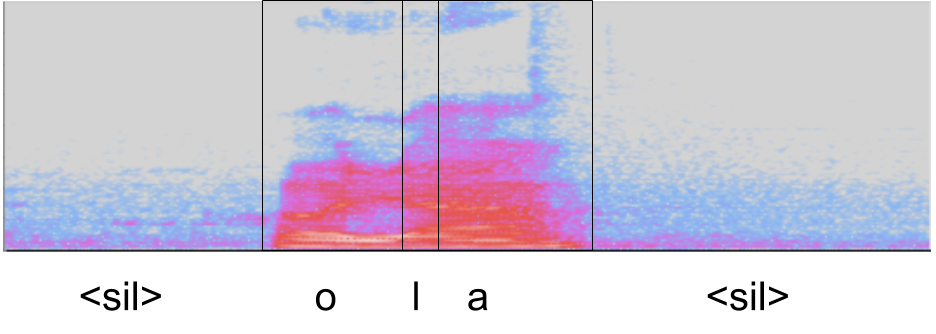
\includegraphics[scale=0.50]{images/alignment.png}
\end{figure}

En la figura \ref{img:alignment} se muestra un espectrograma de frecuencia que representa una señal hablada de la palabra Hola, bajo ella, una alineación fonética.

\section{Representación fonética}

Desde 1888, el Alfabeto Fonético Internacional (International Phonetic Alphabet IPA) es el métidi estándar para representar y clasificar fonemas, indidicando con un alto nivel de precisión las variaciones en la manera de articulación o la localización vocal de las modulaciones. Pequeñas variaciones en los fonemas son llamadas alófonos y pueden aumentar el nivel de anotación  \cite{IPAAlphabet}, pero en la práctica no son usados.
% Since 1888 the International Phonetic Alphabet (IPA) is the standard method to represent and classify phonemes, indicating with a high level of precision small variations of the manner of articulation or location of vocal tract modulations. Little variations on phonemes are called allophones and can improve the level of annotation \cite{IPAAlphabet}, but is not used in practice.

Las vocales son caracterizadas por la posición de la lengua y el tamaño de la abertura de la boca, teniendo diferentes representaciones, que se pueden observar en la tabla \ref{tab:ipa_table_vowels}. 
% Vowels are characterized by the position of the tongue and the wideness of the mouth having different representations variating the position as shown in Table \ref{tab:ipa_table_vowels}. 

Las consonantes están clasificadas en dos segmentos: las pulmónicas, que requieren aire saliendo de los pulmónes y las no pulmónicas, donde no sale aire. En ambas las modificaciones en el tracto bucal definen el sonido. Las consonantes están divididas en dentales, coronales, dorsales y laríngeas, las cuales a su vez están subdivididas en otros sub segmentos. También la manera de articular define el sonido producido, siendo las maneras de articular: plosivas, nasales, oclusivas, fricativas, aproximantes, eyectivas o implosivas.

Vea la clasificación de las consonantes en las tablas \ref{tab:ipa_table_pulmonic_consonants} y \ref{tab:ipa_table_non_pulmonic_consonants}.
% Consonants are classified in pulmonic and non-pulmonic, where modifications on superior vocal tract define the sound. All consonants are segmented in labial which subdivides in bi-labial labio-dental and labio-lingual; coronal divided into dental, alveolar, post-alveolar and retroflex; dorsal divided into palatal, velar, uvular; and laryngeal, divided in  pharyngeal and glottal; each classification can have a relationship with an articulation manner which is plosive, nasal, thrill, tap, flap, fricative, approximant, ejective, click or implosives. 

La representación del Alfabeto Fonético Internacional para las vocales está mostrado en la tabla \ref{tab:ipa_table_vowels}, donde se clasifican los sonidos por su centro silábico y la apertura del tracto bucal.
% IPA representation for vowels are mentioned in table \ref{tab:ipa_table_vowels}, pulmonic consonants are mentioned on table \ref{tab:ipa_table_pulmonic_consonants} and non-pulmonic consonants are mentiones on table \ref{tab:ipa_table_non_pulmonic_consonants}


\begin{landscape}
\begin{table}
\centering
\caption{Alfabeto Fonético Internacional: Consonantes pulmónicas}
\label{tab:ipa_table_pulmonic_consonants}
\begin{tabular}{|p{25mm}|l|p{15mm}|l|l|p{15mm}|l|l|l|l|l|l|}
\hline
{} & Bilabial & Labio\newline dental & Dental & Alveolar & Post-\newline alveolar & Retrofleja & Palatal & Velar & Uvular & Faríngea & Glotal \\
\hline
Plosiva& p b  & & \multicolumn{3}{|c|}{t d} & \textipa{\:t \:d } & \textipa{c \*j} & k g &  q G & & \textipa{P} \\
\hline
Nasal& m &  \textipa{M} & \multicolumn{3}{|c|}{n} & \textipa{\:n}  &  \textipa{\*n}  & \textipa{N} & N &  & \\
\hline
Vibrante& B & & \multicolumn{3}{|c|}{r}  & & & & R &  & \\
\hline
Aproximante & & \textipa{ⱱ} & \multicolumn{3}{|c|}{\textipa{R}} & \textipa{\:r} & & & & &  \\
\hline
Fricativa  & \textipa{F B}& f v & \textipa{T D} & s z & \textipa{S z} & \textipa{\:s \:z} & \textipa{\c{c} J}& x \textipa{G} &\textipa{X  K}  &\textcrh \textipa{Q} & h\textipa{H}  \\
\hline
Lateral \newline fricative& & & \multicolumn{3}{|c|}{\textbeltl \textipa{\*z}} & & & & &  & \\
\hline
Aproximante & & \textipa{V}& \multicolumn{3}{|c|}{\textipa{\!R}} & \textipa{\:R} & j  & \textturnmrleg & & &  \\
\hline
Aproximante lateral& & \multicolumn{3}{|c|}{\textipa{l}} &  \textraisevibyi & \textturny & \textipa{\;L} & & & & \\
\hline
\end{tabular}
\end{table}
\end{landscape}
% \begin{landscape}
\begin{table}
\centering
\caption{Alfabeto Fonético Internacional: Consonantes no pulmónicas}
\label{tab:ipa_table_non_pulmonic_consonants}
\begin{tabular}{|p{20mm}|l|l|l|l|l|l|}
\hline
{} & Bilabial & Dental & Alveolar  & Palatal & Velar & Uvular   \\
\hline
Eyectiva \newline oclusiva& p\textipa{'}  & &t   & c\textipa{'} & k\textipa{'} &  q\textipa{'}  \\
\hline
Eyectiva \newline fricativa& \textipa{F'}  & \textipa{T'}&  s\textipa{'} & \textipa{\c{c}'} & x\textipa{'} & \textipa{X'}  \\
\hline
Click &\textipa{\!o}  & \textipa{|} & \textipa{!} &  & & \\
\hline
Implosiva & \textipa{\!b}  & \multicolumn{2}{|c|}{\textipa{\!d}} &  \textipa{\!j} & \textipa{\!g} & \textipa{\!G} \\
\hline
\end{tabular}
\end{table}
% \end{landscape}
% \begin{landscape}
\begin{table}
\centering
\caption{International Phonethic Alphabet Vowels}
\label{tab:ipa_table_vowels}
\begin{tabular}{|l|l|l|l|l|l|l|}
\hline
{} & \multicolumn{2}{|c|}{Front} & \multicolumn{2}{|c|}{Central} & \multicolumn{2}{|c|}{Back}   \\
\hline
Close & i  & y &\textbaru   & \textbari & \textturnm &  u  \\
\hline
Near close & \textsci  & \textscy &  \multicolumn{2}{|c|}{} &  & \textupsilon  \\
\hline
Close mid & e  & \textipa{\o} &\textreve &  \textbaro & \textramshorns & o \\
\hline
Mid &  \multicolumn{2}{|c|}{} & \multicolumn{2}{|c|}{\textschwa} &  \multicolumn{2}{|c|}{} \\
\hline
Open mid &\textepsilon  & \textipa{\oe} & \textrevepsilon & \textcloserevepsilon  & \textturnv & \textopeno \\
\hline
Near open & \multicolumn{2}{|c|}{\ae} &\multicolumn{2}{|c|}{\textturna} &  \multicolumn{2}{|c|}{}  \\
\hline
Open & a  & \textscoelig &  \multicolumn{2}{|c|}{}  &\textscripta & \textturnscripta \\
\hline
\end{tabular}
\end{table}
% \end{landscape}

Cada idioma utiliza un sub conjunto de los fonemas definidos en este alfabeto fonético.
% Each language uses a subset of phonemes to define its own pronunciation.

Cada palabra de cualquier idioma tiene una y solo una representación fonética, y la relación entre la palabra y esta representación es llamada diccionario fonético. Además de esta representación, son necesarias otras características para representar una señal hablada, como el silencio, los murmullos y otros sonidos que no representan palabras pero añaden información a la grabación del audio.
% Every language's word has only one phonetic representation and the relation between each word and its phonetic representation are called a phonetic dictionary. Besides the phonetic representation of each phoneme other features are needed to represent speech phenomenons like silence, mumbling and other inaudible sounds that can be perceived in a speech recording.

\section{Representación Digital}

Teniendo esta transcripción del audio, el resultado esperado de un Alineador Forzado es una lista de intervalos de tiempo relacionados a cada transcripción entre los cuales cada unidad fonética ocurre.
% Having the transcription of a speech audio the expected output from a FA is a list intervals where phonemes occurs.

Después de entender los principios fonológicos de la voz y su representación abstracta, se presenta una breve descripción de la representación computacional de las señales de voz.
% After understanding the phonological principles and its computational representation, an audio computational representation is also required.

Para representar una señal de voz analógica la manera mas simple y aceptada es la Modulación por Impulsos Codificados (Pulse Code Modulation PCM) por la cual un transductor sensa la onda acústica correspondiente a la señal hablada en intérvalos de tiempo uniformes y los traduce en una escala digital. La calidad de la representación digital depende de la frecuencia de muestreo (cantidad de muestras por segundo) y la profundidad de bits (cantidad de posibles valores digitales tomados en cada muestra). Con esta representación, un audio es solo una lista de valores en un rango determinado donde cada valor representa la presión de aire aplicada al transductor. Este formato es usualmente representado con extensiones .pcm, pero otros formatos de audio crudo son mayormente usados, como la extensión .wav, donde la misma secuencia de valores es almacenada y nombrada como canal, pero con prefijos que indican la frecuencia de muestreo, la profundidad de bits y otros valores específicos como la codificación de cada byte número de canales.
% To digitally represent an analog speech audio a widely accepted way is to use Pulse Code Modulation (PCM) where a transducer senses wave corresponding to the speech on a uniform time interval and translated it in a digital scale. The quality of the digital representation depends on the sampling rate (quantity of measurements by second) and the bit depth (possible digital values to represent each sample). With this representation, an audio is just a list of values in a range that varies representing the pressure applied to a transducer. This format is usually represented with a .pcm extension, but other formats of raw audio exists, like .wav, where the raw audio is stored after a set of headers that defines sampling rate, bit depth, endianness and number of channels.

La representación cruda del audio es útil para reconstruir la señal análoga de una manera mas sencilla, pero para entender la relación entre esta señal digital y su representación fonética es necesario recurrir a técnicas para el procesamiento digital de señales.
% Raw representation of audio is useful to reconstruct easily the analog signal, but to understand the relation between audio segments and phonetic information new ways to represent audio needs to be define.

\section{Técnicas de alineamiento}

Para tener una manera uniforme de representar cada audio, el análisis de frecuencias en cortos periodos de tiempo (Short Time-Frequency Analysis), es una técnica muy usada, la cual consiste en dividir la señal en segmentos uniformes y desfasados en una unidad constante menor a la del tamaño del segmento, buscando que cada segmento se comporte como una señal estacionaria con la cual se pueden extraer parámetros de frecuencia usando transformadas como Fourier o Wavelet, una ilustración de este proceso puede observarse . Esta fase del análisis es conocida como Extracción de Características (Feature Extraction FE) y se usan técnicas como Mel Frequency Cepstral Coefficients (MFCC)\cite{Davis1980ComparisonSentences}, Perceptual Linear Prediction (PLP) \cite{Hermansky1990PerceptualSpeech}, Linear frequency cepstral coefficients LFCC \cite{Davis1980ComparisonSentences}, Wavelet-packet features (WPF) \cite{Farooq2001MelRecognition}, Subband-based cepstral parameters (SBC) \cite{Sarikaya98waveletpacket}, Mixed wavelet packet advanced combinational encoder (MWP-ACE) \cite{NogueiraWaveletImplants} entre otras.

\begin{figure}[H]

\centering
\caption{Extracción de características}
\label{img:fe}
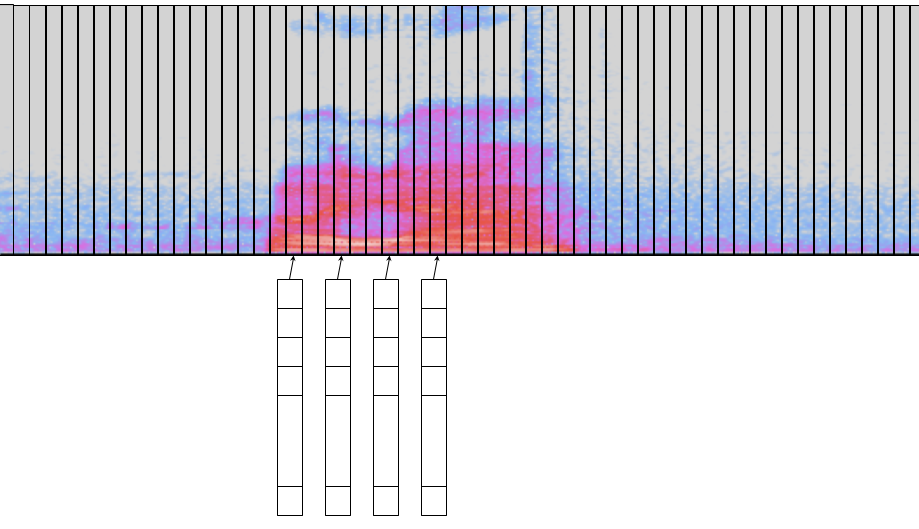
\includegraphics[scale=0.50]{images/fe.png}
\end{figure}

En la figura \ref{img:fe} se muestra un esquema de extracción de características usando un desfase igual al tamaño de la ventana de tiempo de cada segmento. De cada ventana de tiempo se extraen características de la señal que en ese segmentose comporta como una señal estacionaria.
% To have a more uniform way to represent each audio, short time-frequency analysis are used and the technique consists in split the audio in fixed length chunks and each chunk with a defined offset usually less than the chunk length itself, and extract frequency features of each chunk using transforms like Fourier or Wavelet, this phase is usually called Feature Extraction and techniques like Mel Frequency Cepstral Coefficients (MFCC)\cite{Davis1980ComparisonSentences}, Perceptual Linear Prediction (PLP) \cite{Hermansky1990PerceptualSpeech}, Linear frequency cepstral coefficients LFCC \cite{Davis1980ComparisonSentences}, Wavelet-packet features (WPF) \cite{Farooq2001MelRecognition}, Subband-based cepstral parameters (SBC) \cite{Sarikaya98waveletpacket}, Mixed wavelet packet advanced combinational encoder (MWP-ACE) \cite{NogueiraWaveletImplants}.

Con esta nueva representación discreta de la señal hablada, un modelo que identifique los límites entre fonemas suele ser mas claro, pues existe similaridad entre cada segmento de la fase anterior.
% With this new representation a model to identify intervals and boundaries between phonemes are clear, because similar 

Para crear un modelo de alineación de audio las aproximaciones se dividen en 3 grupos: Pliegue Dinámico Temporal (Dynamic Time Warping DTW)  \cite{Sakoe1978DynamicRecognition}, en donde se generan artificialmente señales equivalentes a las esperadas en la señal de audio con la descripción fonética de la misma y luego se calcula una matriz de diferencias entre las señales, buscando valores intermedios que minimicen la diferencia entre ambas señales. La segunda aproximación utiliza Modelos Ocultoss de Markov (Hidden Markov Models HMM) los cuales determinan un modelo probabilístico de transición entre fonemas a partir de datos propiamente anotados para posteriormente con este modelo definir la nueva alineación de las señales propuestas \cite{RabinerARecognition}. La última aproximación utiliza Redes Neuronales Artificiales (Artificial Neural Networks ANN) homogenizando la señal en secuencias de vectores y creando modelos que maximicen la predicción de los fonemas esperados  \cite{Deng2012}.
% To create a model to align speech three major techniques are used, the first is called Dynamic Time Warping (DTW) \cite{Sakoe1978DynamicRecognition} where an artificial wave with the phonetic representation of the annotation is created and then an alignment algorithm minimize the difference using a distance matrix. Another widely used approach is to use HMM where a probabilistic model is created to represent the transition between phonemes and then use this model to align existing waves \cite{RabinerARecognition}. The last approach is ANN using a normalization model to homogenize speech in sequences of vectors and create a model that maximize the prediction of a new vector \cite{Deng2012}.

\subsection{Pliegues Dinámicos Temporales}

Para el DTW la idea principal es eliminar la fluctuación de una señal particular con respecto a una generada sintéticamente creando una normalización temporal donde los fonemas correspondientes ocurren en intervalos te tiempo recurrentes. Para lograr esta normalización, se utilizan algoritmos de programación dinámica para maximizar la coincidencia entre dos patrones de voz. Las transformaciones en el tiempo que se hacen hacen  en ambas señales, son llamadas aproximaciones simétricas y se espera una función objetivo que minimice la distancia entre las dos señales.
% For DTW the main idea es to eliminate the fluctuation of a particular speech creating a time normalization where phonemes occur in a recurrent time interval. To achieve this normalization, dynamic programming algorithms are proposed to generate the maximum coincidence between two speech patterns. Time speech transformations are usually made in both signals, this is called a symmetric approach, and a function that minimizes the distance between both signals is the expected output. 

\begin{figure}[H]

\centering
\caption{Pliegues Dinámicos Temporales \cite{Zhang2017DynamicLength}}
\label{img:dtw}
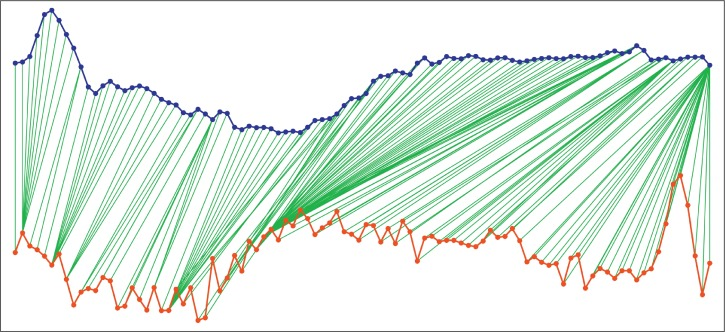
\includegraphics[scale=0.50]{images/dtw.jpg}
\end{figure}

En la figura \ref{img:dtw} se muestra un proceso de pliegue dinámico unidireccional de la señal representada por los puntos rojos a la señal con representada con los puntos verdes.

Generar una señal artificial a partir de la representación fonética de la señal deseada requiere un conocimiento previo de la equivalencia fonética-acústica teniendo modelos basados en reglas que se concatenan para generar la señal objetivo. El proceso de generación de señales acústicas a partir de representaciones fonéticas es llamado Texto a Voz (Text To Speech TTS) y usualmente se obtiene como resultado inverso de un proceso de ASR donde se utiliza el modelo de conocimiento como modelo de generación.
% Generating an artificial wave with the phonetic representation of real speech, where the algorithm know a priori the intervals where each phoneme occurs and minimizing the distance between those two waves, a reconstruction of the real speech wave can be perform using the opposite sequence that minimize the distance between the waves.

\subsection{Modelos Ocultos de Markov}

Alinear una onda usando Modelos Ocultos de Markov requiere un modelo pre existente que defina los estados ocultos de cada modelo de Markov. Esta estimación inicial se realiza por medio del algoritmo Baum-Welchm el cual define unos valores iniciales que pueden ser aleatoreos y los modifica en cada iteración hasta tener una configuración apropiada para las etiquetas y los estados usando un algoritmo de maximización de expectativa (Expectation Maximation EM). La generación de este modelo permite definir una matriz de costos que se puede optimizar por medio del algoritmo de Viterbi para encontrar la secuencia de etiquetas mas probable para la entrada data. En el caso de las señales habladas, la entrada está representada por una secuencia de vectores con características de cada ventana de señal y la salida es su correspondiente secuencia de fonemas.
% Aligning a wave using HMMs requires a preexisting model that defines the hidden states of the markov models. This estimation usually uses a Baum-Welch algorithm, where a set of values are proposed for the hidden layer usually randomly and maximized using an Expectation-Maximization algorithm. This model then allows to use the Viterbi algorithm to find a maximum sequence of probability of hidden states for a new sequence, where the sequence is a speech vector and the hidden state represents the phonemes.

\begin{figure}[H]

\centering
\caption{Modelos Ocultos de Markov}
\label{img:hmm}
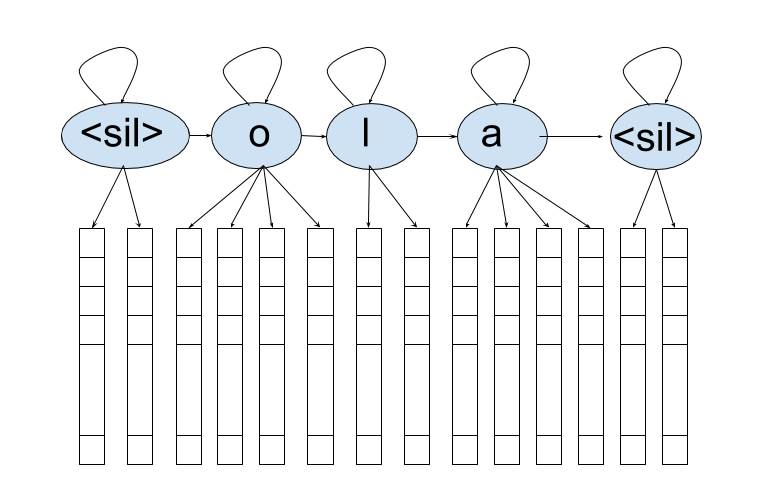
\includegraphics[scale=0.50]{images/hmm.png}
\end{figure}

En la figura \ref{img:hmm} se muestra una posible configuración de estados que representan fonemas y la secuencia de vectores extraidos de la señal hablada

\subsection{Redes Neuronales Artificiales}

Las implementaciones de redes neuronales artificiales para enfrentar el problema de la identificación de secuencias de fonemas a partir de señales habladas es muy variada, existiendo aproximaciones fin-a-fin (End to End) donde se toma directamente la señal cuantizada y por medio de topologías profundas se obtienen modelos aproximados \cite{Hannun2014}. Otras aproximaciones usan algoritmos los extracción de características mencionados anteriormente y en vez de usar los algoritmos de Baum-Welch para parametrizar los Modelos Ocultos de Markov utilizan redes neuronales, en un esquema similar al mostrado en la imagen \ref{img:cd-dnn-hmm}
% ANN approaches uses vectorization to homogenize speech data and generates a network topology that minimize the error of a new vector.

\begin{figure}[H]

\centering
\caption{Redes Neuronales y Modelos de Markov \cite{Deng2012}}
\label{img:cd-dnn-hmm}
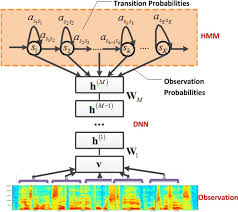
\includegraphics[]{images/cd-dnn-hmm.jpeg}
\end{figure}






\chapter{Estado del arte}
% \section{State of the Art}

\section{Breve historia de los ASR}
% \subsection{A brief history}

El ASR puede ser definido como el proceso mediante el cualo los computadores pueden interpretar señales habladas y producir la representación correspondiente. Este problema se ha atacado desde los años cincuenta, evolucionando desde filtros análigiso donde arreglos específicos de dispositivos físicos extraían información de la señal acústica evaluando frecuencias específicas y comparándolos con grandes bancos de datos \cite{Davis1952AutomaticDigits,Olson1957PhoneticTypewriter}. Esta primera aproximación dió grandes resultados pero poseía las restricciones de ser dependiente del locutor, lo que significa que solo reconoce señales de una sola persona.
% ASR can be defined as the process where computers can interpret speech signals and produce the corresponding text representation. This problem has been addressed since the early fifties and has evolved from analog filters where arrays of specific hardware extract information from the acoustic signal evaluating specific frequencies, compare from a large data bank and output a result  \cite{Davis1952AutomaticDigits,Olson1957PhoneticTypewriter}. This first approach works with high accuracy but was speaker dependent, which means only can recognize words from a single speaker. 

Aproximaciones más sofisticadas se producieron en los sesenta y setenta, donde se cambiaron los filtros análogos por digiltaes y la nosmalización del audio les permitió a los investigadores utilizar Procesamiento Digital de Señales (Digital Signal Processing DSP) y programación dimámica (Dinamic Programming DP) \cite{Velichko1970AutomaticWords,Sakoe1978DynamicRecognition,Itakura1975MinimumRecognition}. Con estas aproximaciones se logró obtener independencia de locutor y reconocimiento de pequeños vocabularios con palabras aisladas.
% More sophisticated approaches were produce in the sixties and seventies where software filters and normalization let researchers work with Digital Signal Processing (DSP) and dynamic programming \cite{Velichko1970AutomaticWords,Sakoe1978DynamicRecognition,Itakura1975MinimumRecognition}, with those approaches speaker independent isolated word recognition with a high accuracy over a small controlled language.

Incrementar el reconocimiento sobre el tamaño del vocabulario fue un problema atacado en la década d elos ochentas y noventas, donde las aproximaciones usando Modelos Ocultos de Markov tomaron mucha fuerza \cite{RabinerARecognition} y se convirtieron en las implementaciones estándares. Otras aproximaciones usando Redes Neuronales Artificiales resultaron menos efectivas \cite{Waibel1989PhonemeNetworks} pero igualmente usadas. Como resultado de la popularidad del problema y los buenos resultados obtenidos, se desarrollaron herramientas y aplicaciones como SPHINX de la Universidad Carnegie Mellon (CMU) \cite{Lee1990AnSystem}, BYBLOS \cite{ChowBYBLOS:System}, el Lincoln Robust Speech Recognizer \cite{PaulTheRecognizer} y el MIT Summit Speech Recognition System \cite{Zue1989TheReport}. La mayoría de estas herramientas usan Modelos Ocultos de Markov en combinación con Modelos de Mixturas Gausianas usando senones: una sub unidad finéntica la cual le permite a cada fonema tener varios estados de transición para luego ser agrupados en un modelo único.
% Increasing the vocabulary size was a problem addressed in the eighties and nineties where approaches like Hidden Markov Models (HMM) \cite{RabinerARecognition} and Artificial Neural Networks (ANN) \cite{Waibel1989PhonemeNetworks} won popularity as methods to treat large vocabularies. A result of this popularity many software frameworks where develop like SPHINX by Carnegie Mellon University (CMU) \cite{Lee1990AnSystem}, BYBLOS \cite{ChowBYBLOS:System}, the Lincoln Robust Speech Recognizer \cite{PaulTheRecognizer} and the MIT Summit Speech Recognition System \cite{Zue1989TheReport}. Many of these systems use an HMM approach mixed with a Gaussian Mixture Models using Senones: a sub-phonetic unit which allows each phone sub model to share and cluster its state\cite{Hwang}.

Todos estas herramientas ha mostrado grandes resultados en ambientes con reuido reducido, lo cual representa un nuevo reto: mejorar la precición en canales ruidosos, con lo que se inicia una nueva área de investigación denominada Reconocimiento del Habla Robusto (Robust Speech Recognition) \cite{SieglerOnSystems,MirghaforiTowardsASR}. El cual include investigacieon relacionada con el ancho de banda de la perceicpón del sonido y la creción de modulaciones a los espectrogramas de frecuencias para reducir la reverberación y la percepción del ruido \cite{Kingsbury1998RobustSpectrogram}, la segmentación del audio para la identificación de segmentos no confiagles usando marginalización y imputación de datos basado en estado y límites de energía \cite{Cooke2001RobustData} y aproximaciones hibridas  que mejoran la precisión usando combinaciones de Modelos Ocultos de Markov y Redes Neuronles Artificiales \cite{BourlardABands}.
% All these framework shows great results on noise reduced environments, introducing a next challenge: improve accuracy on noisy channels, which starts the concept of Robust Speech Recognition \cite{SieglerOnSystems,MirghaforiTowardsASR}. Which includes research in reducing bandwidth of the sound perception and create a modulation spectrogram to reduce reverberation and noise perception \cite{Kingsbury1998RobustSpectrogram}, segment the audio wave and identify unreliable segments using marginalization and state-based data imputation combined with energy bounds which improved performance on noisy channels \cite{Cooke2001RobustData} and new hybrid approaches to improve performance combining existing HMM with ANN \cite{BourlardABands} to mention some relevant areas.

La introducción de las Unidades de Procesamiento Gráfico (Graphical Unit Processors GPS) para acelerar los procesos de aprendizaje automático en clasificación de imágenes \cite{KrizhevskyImageNetNetworks} también impacto el ASR, dando un nuevo impulso a las técnicas hibridas y de redes neuronales, donde una aproximación que tomó mucha fuerza fue la de Redes Neuronales Profundas Dependientes de Contexto con Modelos Ocultos de Markov (Context-Dependent Deep Neural Network Hidden Markov Model CD-DNN-HMM) \cite{Yu_2014_1,Xiong2017}  y también aproxmiaciones que usan únicamente técnicas de aprendizaje profundo \cite{Povey_ASRU2011,1401.6984}.
% Introduction of Graphical Unit Processors (GPU) to accelerate machine learning algorithms for Image Classification \cite{KrizhevskyImageNetNetworks} also impact ASR, giving a new a rise of hybrid techniques using Context-Dependent Deep Neural Network Hidden Markov Model (CD-DNN-HMM) \cite{Yu_2014_1,Xiong2017} and also new frameworks based on Deep Learning techniques \cite{Povey_ASRU2011,1401.6984}.

%  El estado del arte, es una revisión de literatura (Internet, libros, revistas,etc) que permite identificar que otros trabajos similares hay en el área, o cuál es el borde del conocimiento que nos permite realizar la propuesta. Esta sección no debe superar una hoja. Tome lo desarrollado previamente y haga una sintesis.

\section{Herramientas existentes}
% \section{Existing tools}

Muchos Alineadores Forzados de código abierto utilizan investigación teórica para materializar la alineación de recursos existentes. Basada en la categorización mencionada previamente, se agrupan alineadores existentes en las siguientes categorías

\begin{itemize}
    \item Pliegues Dinámicos Temporales
    \item Modelos Ocultos de Markov
    \item Redes Neuronales Artificiales
\end{itemize}
% Open source forced aligners uses theoretical research to create tools to materialize alignment on existing resources. Based on previously mentioned categorization the existing aligners are grouped in the categories: Dynamic Time Warping, Hidden Markov Models and Artifical Neural Networks.

\subsection{Pliegues Dinámicos Temporales}
% \subsection{Dynamic Time Warping}

Para DTW la idea principal es generar señales de voz artificiales utilizando software de tipo grafema a fonema, también conocido como texto a vos (Text To Speech TTS), y luego aliear la señal de entrada con la generada artificialmente.

% For DTW the main idea is to generate an artificial speech using Grapheme to Phoneme  software and then align the input speech with the artificially generated wave

\textbf{Aeneas}.

Aneneas \cite{aeneas} es un software desarrollado por Alberto Pettarin para Read Beyond, un software de audio libros, liberado bajo licencia GNU Affero General Public Licence versión 3 (AGPL v3) en 2015, con varias actualizaciones hasta 2017. Para la generación de la señal artificial, Aeneas usa eSpeak \cite{espeak}, otro software licenciado bajo la licencia GNU Public Licence (GPL) por the Free Software Foundation. eSpeak en su versión original soporta mas de 28 lenguajes, incluyendo Inglés y Español
% Aeneas \cite{aeneas} uses espeak \cite{espeak} to generate the base generates speech wave. Then align the input word using dynamic programming.

\subsection{Modelos Ocultos de Markov}
% \subsection{Hidden Markov Models}

Los Modelos Ocultos de Markov usan una serie de algoritmos para parametrizar los modelos, entre los cuales se destagan el algoritmo de Viterbi para la decodificación \cite{Forney1973TheAlgorithm} y el algoritmo Baum-Welch para la estimación inicial de parámetros.

Este conjunto de algoritmos son implementados por paquetes especializados para el reconocimiento automático del habla, como  HTK \cite{Young1994ThePhilosophy}, Julius \cite{LeeEurospeechEngine} y CMU Sphinx \cite{Lee1990AnSystem}. Estas implementaciones abiertas de algoritmos son usadas por algunas herramientas mostradas a continuación.
% Work with HMM uses a basic set of algorithms where the Viterbi algorithm \cite{Forney1973TheAlgorithm} and the Baum Welch Algorithm. These set of algorithms are implemented for ASR in frameworks and toolkits like HTK \cite{Young1994ThePhilosophy}, Julius \cite{LeeEurospeechEngine} and CMU Sphinx \cite{Lee1990AnSystem}.

\textbf{MAUS}
El Segmentador Automático de Munich (Munich AUtomatic Segmentation) desarrollado por el Instituto de Fonética y procesamiento de señales de la Universidad de Munich está construido usando herramientas de decodificación de HTK y BALLON un sistema de grafemas a fonemas también desarrollado por la  universidad de Munich. Este paquete fue desarrollado en 1994 por Uwe Reichel y Florian Schiel licenciado para propósitos no comerciales y académicos. \cite{WesenickAPPLYINGPRONUNCIATION}. 
% The Munich Automatic Segmentation \cite{WesenickAPPLYINGPRONUNCIATION} is a build on top of HTK and BALLON a Grapheme to Phoneme Suite created by Uwe Reichel and uses a hybrid approach between DTW and HMM

\textbf{SPPAS}
SPPAS es un anotador automático y analizador de habla es una herramienta de computación científica desarrollada para proveer un análisis fonético robusto y confiagle \cite{Bigi2016ASPPAS}. Fue creada por Brigitte Bigi  en el Laboratorio del habla y la lengua (Laboratoire Parole et Langage) de Francia, licenciado con la licencia GPL v3, utiliza Julius para el procesamiento de los Modelos Ocultos de Markov.
% SPPAS \cite{Bigi2016ASPPAS} is a suite for automated for automated annotation and speech analysis created by Brigitte Bigi at Laboratoire Parole et Langage in France and uses Julius for HMM processing and Viterbi Algorithm

\textbf{Prosodylab Aligner}
Prosodylab Aligner \cite{Gorman2011Prosodylab-aligner:Speech} fue creado en el Laboratorio de Prosodia (Prosody Lab) en la Universidad de Mcgill en Canada, por Kyle Gorman y está compuesta de una serie de herramientas y scripts para crear alineaciones usando HTK cusando monófnos para entrenar sus modelos.
% Prosodylab Aligner \cite{Gorman2011Prosodylab-aligner:Speech} was created at Prosody Lab in Mcgill University by Kyle Gorman and are composed by a set of tools of scripts to create alignment using HTK as backend using mono-phones to train its models

\subsection{Redes Neuronales Artificiales}
% \subsection{Artificial Neural Networks}

Los anotadores de código abierto basados en redes neuronales utilizan Kaldi \cite{Povey_ASRU2011}, un paquete diseñado por Daniel Povey en el instituto universitario John Hopkings, y licenciado bajo la licencia Apache 2.
% For ANN the Kaldi toolkit \cite{Povey_ASRU2011} is used to improve development times.   

\textbf{Gentle Forced Aligner}

Gentle \cite{gentle} es un alineador forzado construido a partir de un modelo de bigramas y conceptos de programación dinámica para alienar el audio.
% Gentle \cite{gentle} is a FA build on top of Kaldi. The main approach is to use a web server to evaluate an input speech. The model uses dynamic programming to align audio using a bigram model

\textbf{The Montreal Forced Aligner}

El Alineador Forzado de Montreal, fue creado en la Universidad de Mcgill en el laboratorio de prosidia \cite{McAuliffe2017MontrealKaldi}, licenciado con la licencia MIT  como una versión mejorada de Prosylab Aligner, utilizando el corpus GlobalPhone  para crear modelos trifónicos que mejoran el rendimiento con respecto al alineador anterior.
% The Montreal Forced Aligner \cite{McAuliffe2017MontrealKaldi} was created at Prosody Lab in Mcgill University as the evolution for Prosodylab Aligner. It uses Kaldi as backend and Globalphone to create a triphone model that improves performance comparing Prosodylab Aligner
\chapter{Cronograma}
% \section{State of the Art}

Para el desarrollo de las actividades relacionadas con los objetivos, se estima un tiempo de trabajo de doce meses separando las actividades en cuatro grandes fases:

\begin{itemize}
    \item Estudio de alineadores forzados 
    \item Recolección de recursos anotados
    \item Diseño e implementación 
    \item Anotación de corpus existentes
\end{itemize}

Se inicia con un mes dedicado al análisis del arte, contemplando el análisis de los alineadores abiertos existentes, los corpus abiertos anotados y los corpus abiertos no anotados.

Finalizado el estado del arte, se dedican tres meses para el estudio de los alineadores automáticos abiertos, separando un mes para la adecuación de ambientes y puesta en marcha de los alineadores abiertos existentes, entendiendo las técnicas y tecnologías relacionados con cada uno, buscando seleccionar la mejor aproximación para la implementación propia y los últimos dos meses para el análisis teórico de los propuestas de alineadores forzados. Con estas actividades se cierra la primera fase de estudio de los alineadores forzados, teniendo en este punto un análisis comparativo de las herramientas existentes, así también como una visión nocional de los corpus anotados y no anotados abiertos.

La fase dos toma dos meses para el análisis en profundidad de los corpus abiertos anotados y no anotados para el lenguaje español, entendiendo en cada uno sus características de duración y locutores, el nivel de anotación en caso de los anotados y características prosódicas que pueden ser relevantes para la anotación automática posterior. Al final de esta etapa se tendrá un documento descriptivo a profundidad de los recursos abiertos anotados y no anotados para el lenguaje español.

En la fase tres se dedicarán tres meses para la implementación del alineador forzado, teniendo como base de pruebas corpus anotados a un nivel fino, siendo lo ideal una anotación a nivel fonético. Se realizará el desarrollo de forma iterativa iniciando con corpus sin ruido y mejorando la robustés del alineador en ambientes ruidosos. Al final de esta etapa existirá un nuevo alineador forzado de código abierto que miniza la diferencia entre los intervalos de anotación detectados con respecto a los especificados en los corpus anotados seleccionados.

La última fase usa el alineador previamente implementado y realiza una anotación en un corpus abierto de larga duración en el lenguaje español. Se realizarán los ajustes necesarios para una buena anotación de este corpus y se liberará la anotación para ser usada en posteriores investigaciones.

Se muestra un diagrama de Gantt con los estimados de tiempos para cada actividad en la figura \ref{img:schedule}

\begin{landscape}
\begin{figure}[H]

\centering
\caption{Cronograma}
\label{img:schedule}
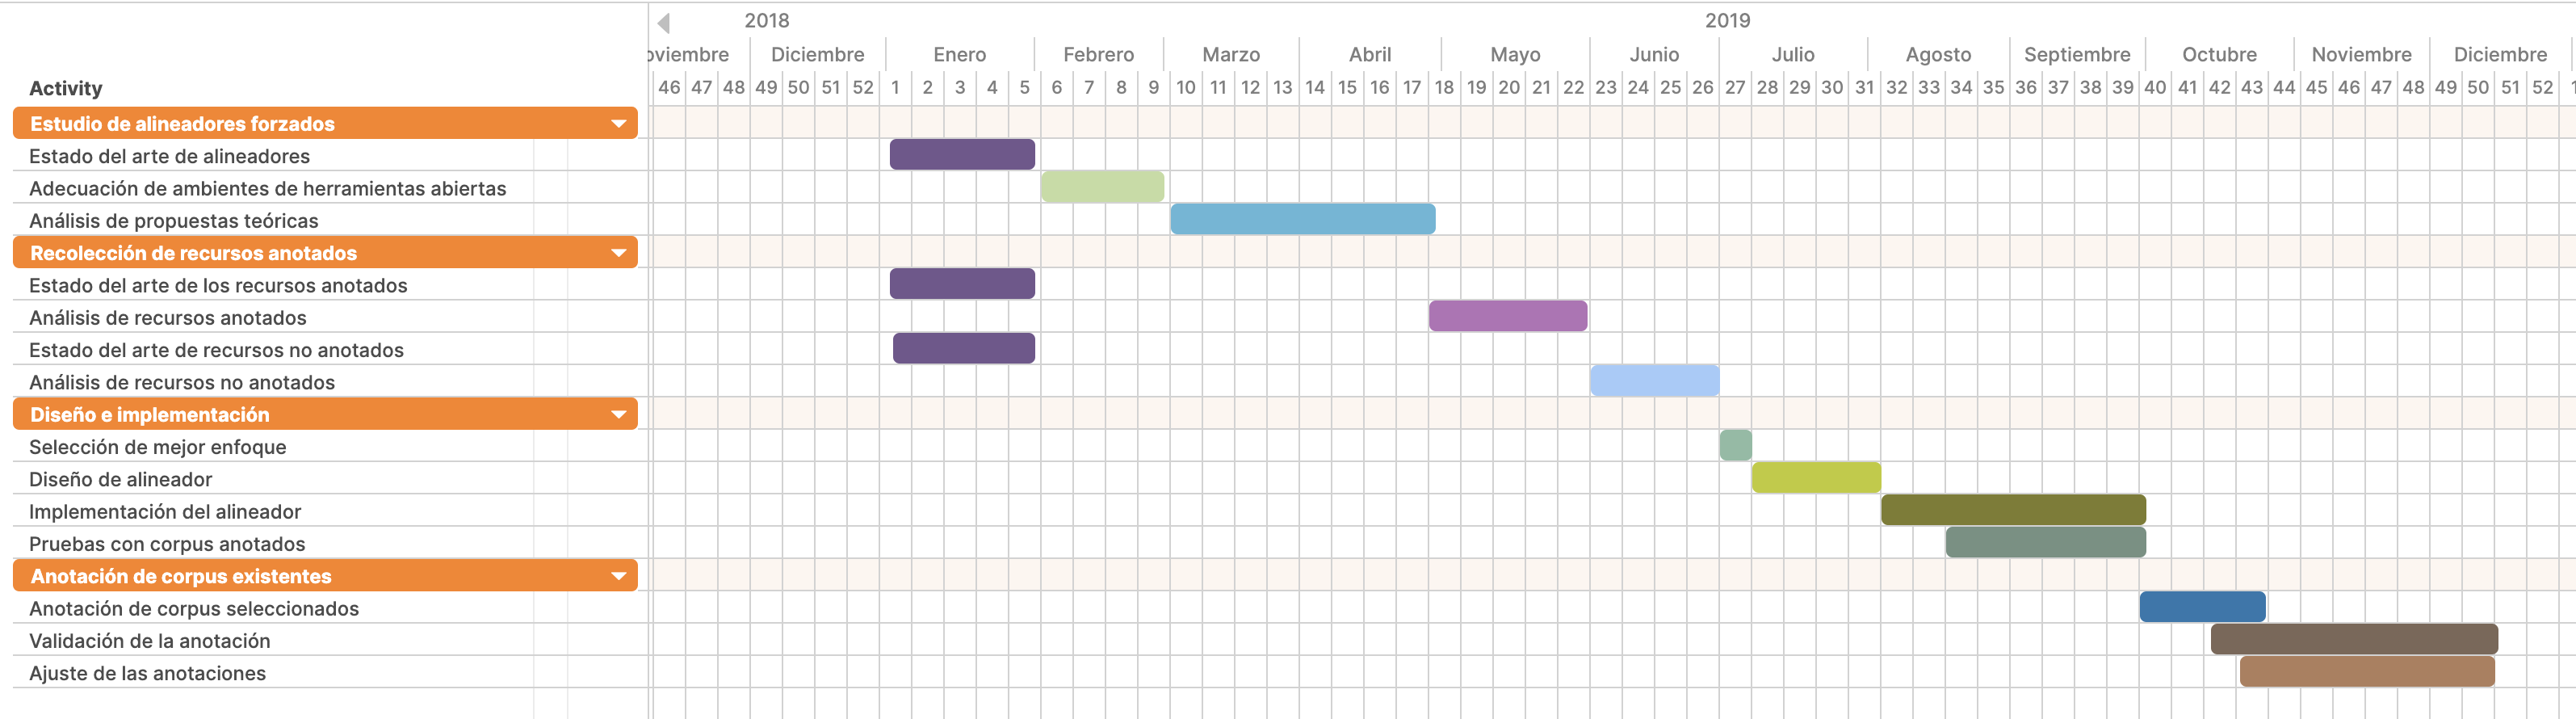
\includegraphics[scale=0.40]{images/schedule.png}

\end{figure}
\end{landscape}
\chapter{Costos}
% \section{Costos}

Para el desarrollo del proyecto, cuya duración se estima de 12 meses, se plantea una estructura de costos considerando el costo de hora del investigador principal, su asesor de tesis y horas hombre de validación manual de la anotación automática como proceso de verificación del corpus anotado automáticamente como costos de recurso humano. También se consideran costos de infraestructura, que contemplan una estación de cómputo para el investigador principal así como recursos en nubes públicas para el alojamiento de aplicaciones web relacionadas con el proyecto. También se espera que como resultado del proyecto se publique un artículo en una revista indexada y se participe en un congreso internacional, para lo cual se estiman los costos de viáticos y honorarios de la casa publicadora. También se estima un presupuesto relacionado con materiales bibliográficos pagos que deban adquirirse en el proceso del proyecto. 

Se detallan los costos estimados en la Tabla \ref{tab:cost_structure}



\begin{table}[]
\centering
\caption{Presupuesto}
% \caption{Speech English Corpus}
\label{tab:cost_structure}
\begin{tabular}{|l|l|l|l|}
\toprule
Cantidad                                   & Cantidad       & Valor Unitario   & Total          \\
\hline
Horas de investigación                     & 1056           & 25000   & 26400000 \\
\hline
Horas director de tesis                    & 52             & 100000  & 5200000  \\
\hline
Horas validación manual                    & 240            & 5600    & 1344000  \\
\hline
Equipo de cómputo                          & 1              & 7500000 & 7500000  \\
\hline
Alojamiento mensual de recursos en la nube & 12             & 100000  & 1200000  \\
\hline
Publicaciones                              & 1              & 1800000 & 1800000  \\
\hline
Conferencias                               & 1              & 4000000 & 4000000  \\
\hline
Material Bibliográfico                     & 1              & 2000000 & 2000000  \\
\hline
Total                                      &                &         & 49444000 \\
\hline
\end{tabular}
\end{table}
% \input{background/background}

% body of thesis comes here

% \input{conclusion/conclusion}

% \appendix
% appendices come here


\addcontentsline{toc}{chapter}{Bibliography}
\bibliographystyle{plain}
% \bibliographystyle{apacite}
% \bibliography{bibliography/bibliography}
\bibliography{references.bib,custom_references.bib}




\end{document}